\documentclass[UTF8,12pt]{article}
\usepackage[utf8]{inputenc}
\usepackage[T1]{fontenc}
\usepackage{vmargin} % page format
\usepackage{soul}       % underline multiple lines
\usepackage{enumerate}
\usepackage{enumitem}
\usepackage{color}
\usepackage{amsmath}
\usepackage{multirow}
\usepackage{amssymb}
\usepackage{bbm}
\usepackage{graphicx}
\usepackage{subfig}
\usepackage{diagbox}
\usepackage[pdfstartview=FitH,
CJKbookmarks=true,
bookmarksnumbered=true,
bookmarksopen=true,
colorlinks=true,                        
linkcolor=black]{hyperref}
\usepackage[numbers]{natbib}
\newcommand{\sinc}{\mathrm{sinc}}
\setpapersize{USletter}
\setmarginsrb{1 in}{1 in}{1 in}{0.5 in}{0pt}{0mm}{0pt}{0.5 in}
\pagestyle{empty}
\pagestyle{plain}
\setlength{\parskip}{1em}
\renewcommand{\baselinestretch}{1.5}
\usepackage{sectsty}% section font size
\usepackage{titlesec}% section spacing
\sectionfont{\fontsize{12}{0}\selectfont}
\subsectionfont{\fontsize{12}{0}\selectfont}
\titlespacing\section{0pt}{12pt plus 4pt minus 2pt}{0pt plus 2pt minus 2pt}
\titlespacing\subsection{0pt}{12pt plus 4pt minus 2pt}{0pt plus 2pt minus 2pt}
\titlespacing\subsubsection{0pt}{12pt plus 4pt minus 2pt}{0pt plus 2pt minus 2pt}

\title{Predicting Hand-written Digits using Principal Components Analysis (PCA)}
\date{2019\\ February}
\author{Yue WU\\ CS 391L}
\begin{document}
	\maketitle
	\section{Introduction}
	This homework aims at using principal components analysis (PCA) to detect hand-written digits automatically. We will use a certain amount of training images included in a training set of 60000 images to derive an algorithm that can detect the digits shown in a test set of 10000 images. x denotes the number of pixels in each images. In this case, x equals to 28*28, which is 784.
	\section{Methods}
	In the implementation, we first calculated the covariance matrix C (x-x or k-k depending on which one is smaller) and mean value vector m (with length x) using k training images stored in matrix A (x-k) (Equation \ref{eq:covariance matrix}), and then we find the eigendigits of the covariance matrix C and store the eigenvectors in matrix V by sorting their corresponding eigenvalues in a descending order. The process is shown in the code namely "hw1FindEigendigits.m". Note that in order to accelerate the calculation, usually we first calculated the eigendigits of the smaller system, and then transfer the eigendigits into the larger system. In our case here we do not need this step because the sizes of the images are small, so we are already doing calculations in a small system.
	\begin{equation}
	\label{eq:covariance matrix}
	C = A*A^{T}
	\end{equation}
	
	The eigenvectors indicate key features found by analyzing k training images. Showing here in Figure \ref{fig:eigens}are the first and third eigenvectors with yellow denoting positive values and blue denoting negative values. Each image can be seen as a weighted combination of these eigenvectors.
	\begin{figure}[!ht]
		\centering
		\subfloat[]{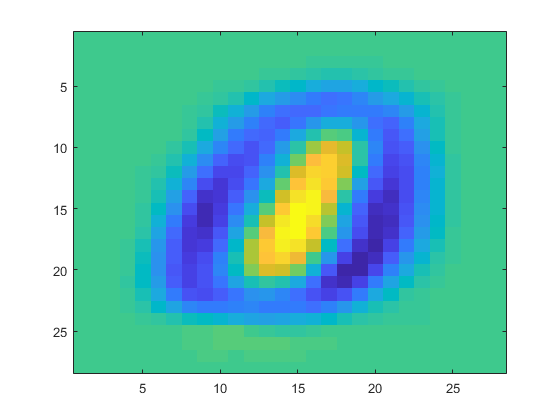
\includegraphics[width=0.5\linewidth]{figures/0_evec_0.png}\label{fig:eigen1}}
		\subfloat[]{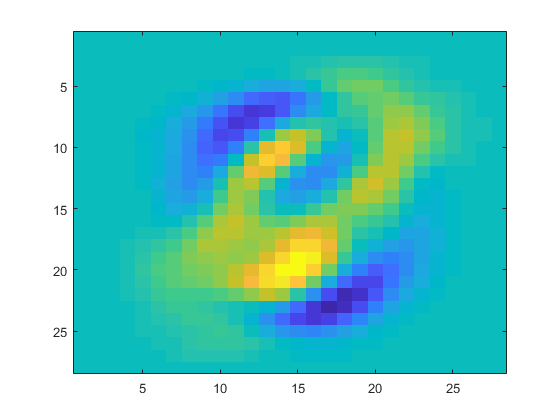
\includegraphics[width=0.5\linewidth]{figures/0_evec_2.png}\label{fig:eigen2}}
		\caption{\label{fig:eigens}(a) (b) The first and third eigenvectors with yellow denoting positive values and blue denoting negative values.}
	\end{figure}
	
	With eigenvectors stored in V and the mean vector m calculated using the training set, we were able to project test images into the eigenspace and find out how each image corresponds to the features preserved in the eigenvectors. In order to test if our eigenvectors are working correctly, we displayed the first two images in the test set, projected them to the eigenspace using Equation \ref{eq:recons1}, and then reconstructed the two images using Equation \ref{eq:recons2}. Here we used 2000 training samples and the first 30 eigenvectors. As is depicted in Figure \ref{fig:recons}, the images reconstructed from the eigenspace are not the same as the original images, but we are still able to tell the main feature of the original images from the reconstruction.
	\begin{equation}
	\label{eq:recons1}
	I' = transpose(I-m)*V
	\end{equation}
	\begin{equation}
	\label{eq:recons2}
	I'' = V*transpose(I')+m
	\end{equation}
	\begin{figure}[!ht]
		\centering
		\subfloat[][]{
\includegraphics[width=.1\textwidth]{figures/1_before_reshape_1.png}}\quad
		\subfloat[][]{
\includegraphics[width=.1\textwidth]{figures/1_before_reshape_2.png}}\\
		\subfloat[][]{
\includegraphics[width=.1\textwidth]{figures/1_after_reshape_1_ntrain2000_neig30.png}}\quad
		\subfloat[][]{
\includegraphics[width=.1\textwidth]{figures/1_after_reshape_2_ntrain2000_neig30.png}}
		\caption{\label{fig:recons}(a) (b) Original test images. (c) (d) Reconstructed images.}
	\end{figure}

	After that, we used the Matlab function \textit{fitcknn} to classify training images into ten classes using the Euclidean distance metric. We set the number of neighbors to be 5. By applying this classification algorithm to the test set, we were able to predict content in each test image and calculate how the accuracy of the prediction changes with different numbers of training samples and different numbers of eigenvectors used.
	\section{Results}
	\begin{figure}[!ht]
		\centering
		\subfloat[]{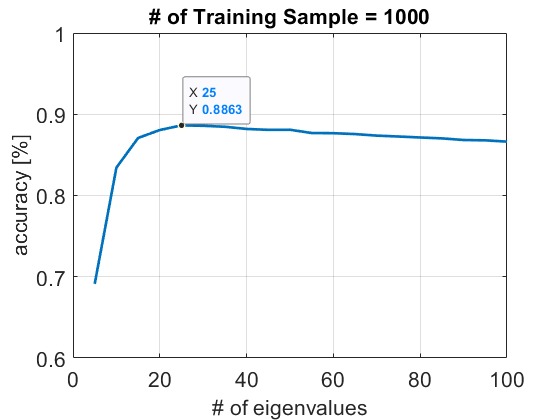
\includegraphics[width=.4\textwidth]{figures/2_ntrain1000.png}}\quad
		\subfloat[]{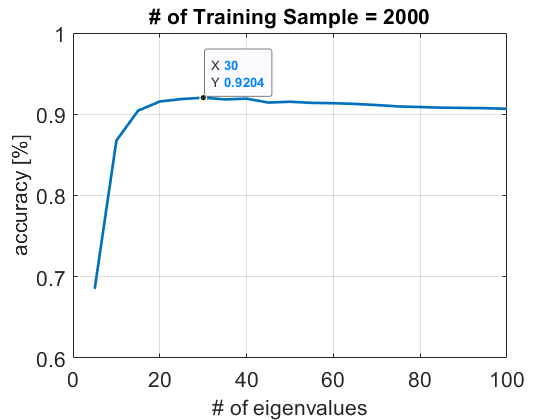
\includegraphics[width=.4\textwidth]{figures/2_ntrain2000.png}}\\
		\subfloat[]{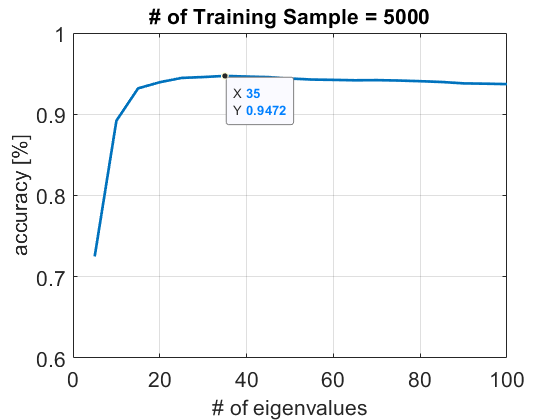
\includegraphics[width=.4\textwidth]{figures/2_ntrain5000.png}}\quad
		\subfloat[]{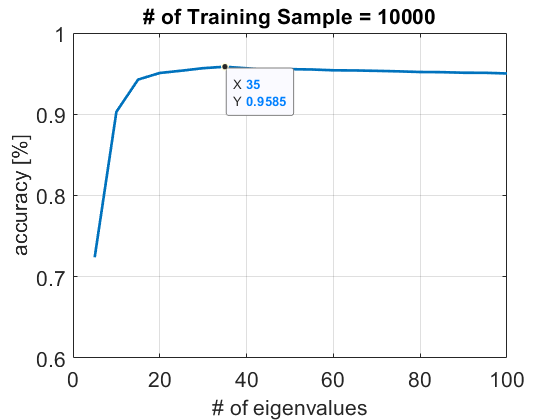
\includegraphics[width=.4\textwidth]{figures/2_ntrain10000.png}}\\
		\subfloat[]{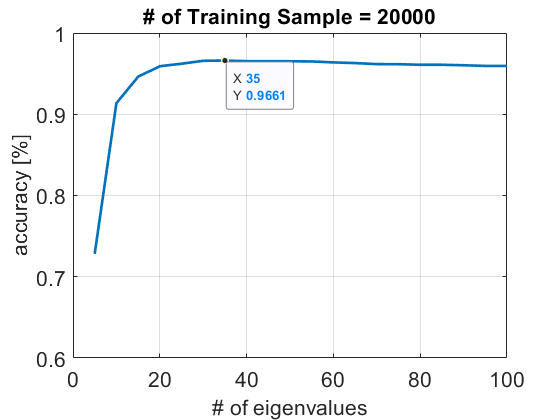
\includegraphics[width=.4\textwidth]{figures/2_ntrain20000.png}}\quad
		\subfloat[]{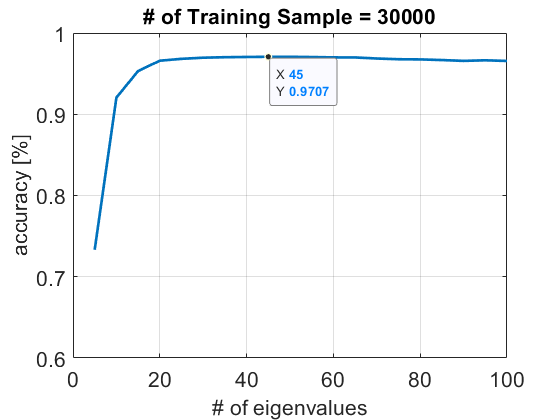
\includegraphics[width=.4\textwidth]{figures/2_ntrain30000.png}}\\
		\caption{\label{fig:accuracy} Accuracy changes with different numbers of training samples: (a) 1000 samples, (b) 2000 samples, (c) 5000 samples, (d) 10000 samples, (e) 20000 samples, (f) 30000 samples, and different numbers of eigenvectors used: from 5 to 100.}
	\end{figure}
	By applying numbers of training samples ranging from 1000 to 30000, and applying numbers of eigenvectors ranging from 5 to 100, we calculated the accuracy changing shown in Figure \ref{fig:accuracy}. As the number of training samples increases, accuracy increases as well. For the same number of training samples, we observe maximum accuracy when the number of eigenvectors used lies between 25 to 45. The optimal number of eigenvectors used increases with an increase in the number of training samples. The optimal number of eigenvalues used for different numbers of training samples as well as the corresponding accuracy are shown in Table \ref{table:accuracy}.
	\begin{table}[]
		\begin{tabular}{l|l|llllll}
			\hline
			&    & \multicolumn{6}{c}{\# of Training Sample}           \\\hline
			&    & 1000   & 2000   & 5000   & 10000  & 20000  & 30000  \\\hline
			\multirow{5}{*}{Optimal \# of Eigenvalues} & 25 & 0.8863 &        &        &        &        &        \\
			& 30 &        & 0.9204 &        &        &        &        \\
			& 35 &        &        & 0.9472 & 0.9585 & 0.9661 &        \\
			& 40 &        &        &        &        &        &        \\
			& 45 &        &        &        &        &        & 0.9707 \\\hline
		\end{tabular}
	\caption{\label{table:accuracy}The optimal number of eigenvalues used for different numbers of training samples as well as the corresponding accuracy.}
	\end{table}
	\section{Conclusion}
	In order to achieve better performance, we should balance between accuracy and the time cost by changing the number of training samples. More training samples make the procedure slower but can increase the accuracy of the prediction. Once we decide the number of training samples we are going to use, we need to find the optimal number of eigenvectors in order to achieve higher accuracy. We will not have enough features to help us decide which class to put the new image into if we use too little eigenvectors, so, the accuracy can be very low with too little eigenvectors. However, too many eigenvectors will disturb the prediction as well because eigenvectors with small eigenvalues are nearly useless. Therefore, it is critical for us to test and find out the optimal number of eigenvectors to use. 

\end{document}